\documentclass{bmstu}

\usepackage{pdfpages}

\addbibresource{inc/biblio/sources.bib}

\begin{document}

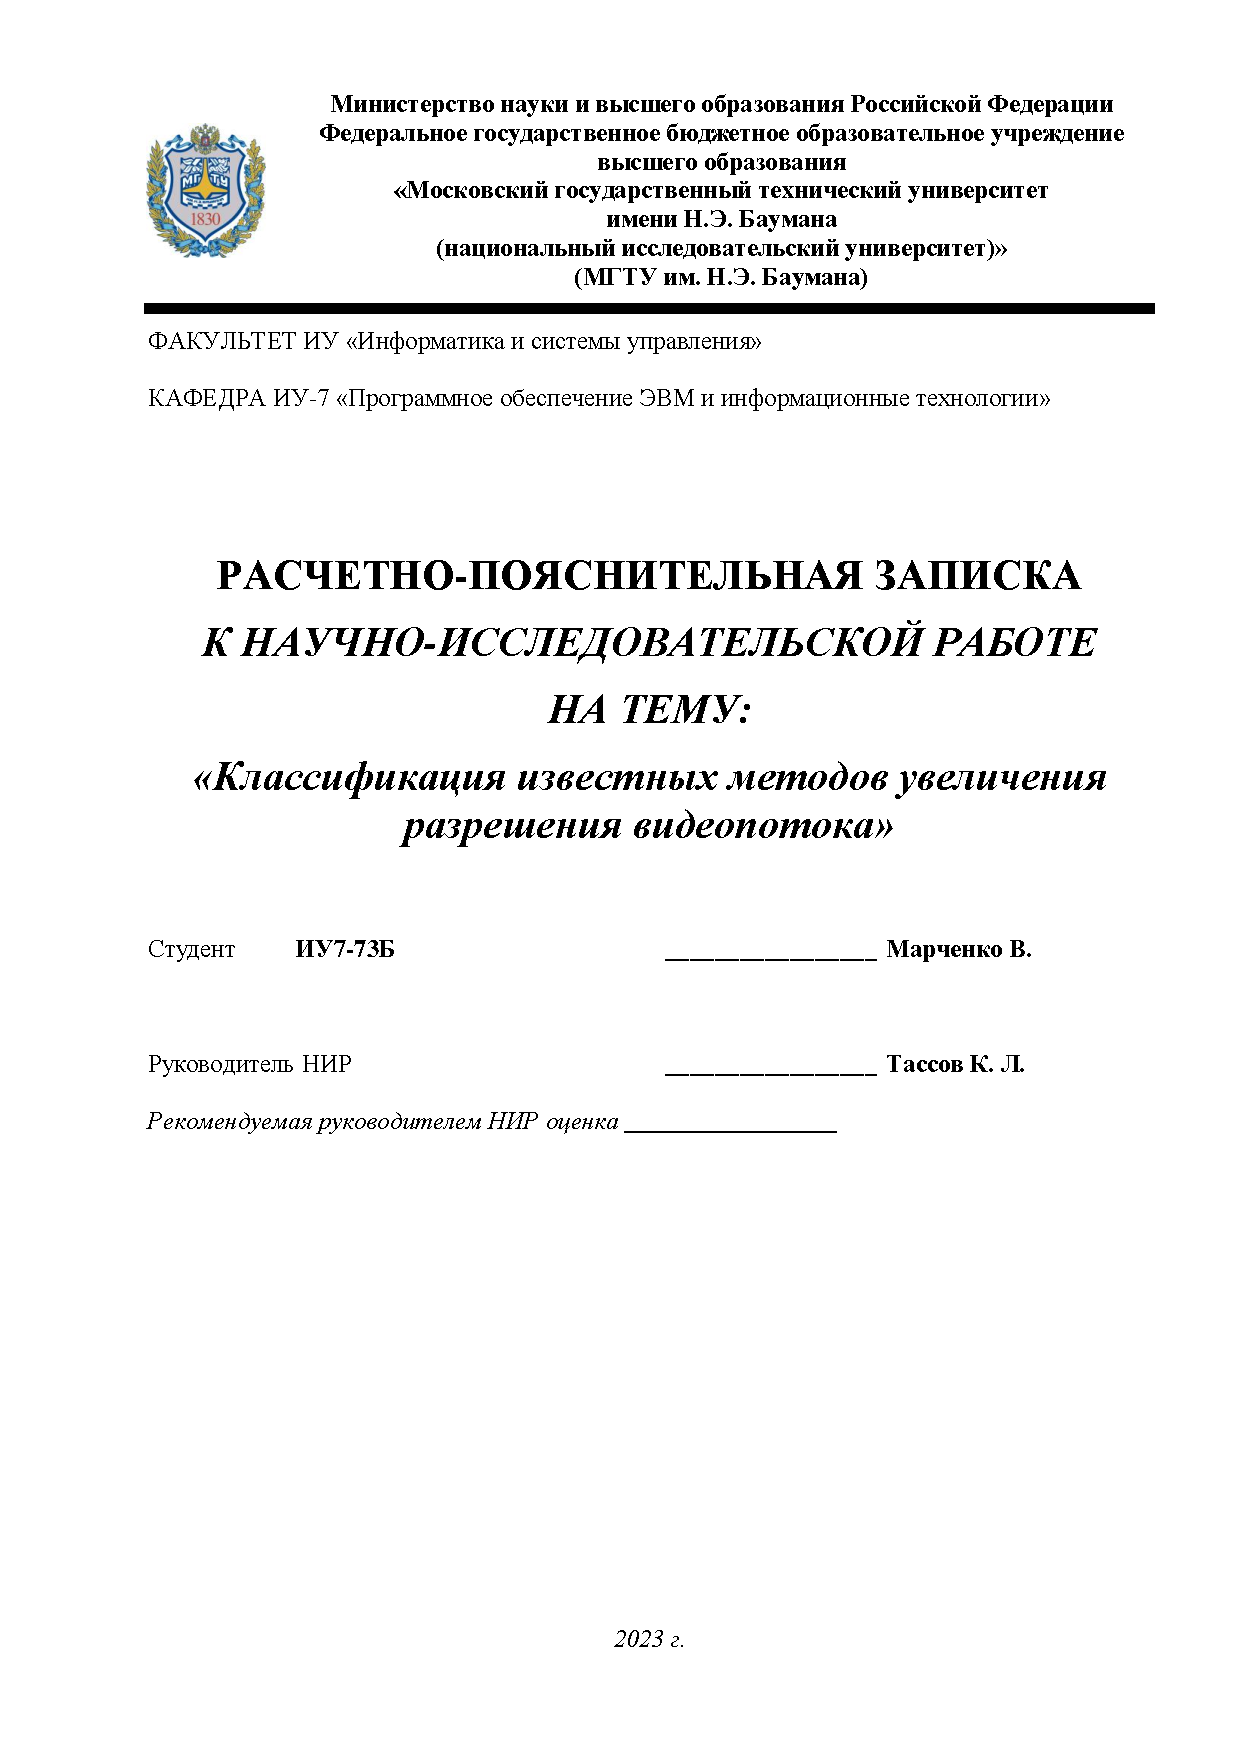
\includepdf[pages=-]{inc/img/title.pdf}

\setcounter{page}{3}

{\centering \chapter*{РЕФЕРАТ}}

Отчет X с., X рис., X табл., X источн., X прил.

\noindent ВИДЕО, ВИДЕОПОТОК, ВИДЕОИЗОБРАЖЕНИЕ, РАЗРЕШЕНИЕ, НЕЙРОННЫЕ СЕТИ

Объектом исследования являются методы увеличения разрешения видеопотока.

Цель работы: классификация известных методов увеличения разрешения видеопотока.

В результате исследования было проведено сравнение ... по ... критериям.

Область применения результатов --- ...

Результат работы...

\maketableofcontents

{\centering \chapter*{ПЕРЕЧЕНЬ СОКРАЩЕНИЙ И ОБОЗНАЧЕНИЙ}}

В настоящем отчете о НИР применяют следующие сокращения и обозначения:

\begin{table}[H]
\begin{tabular}{p{3cm}p{13.5cm}}
VSR & Суперразрешение видео (Video Super-Resolution)
\tabularnewline
SISR & Суперразрешение фото (Single-Image Super-Resolution)
\tabularnewline
DFT & Дискретное преобразование Фурье (Discrete Fourier Transform)
\tabularnewline
DCT & Дискретное косинусное преобразование (Discrete Cosine Transform)
\tabularnewline
DWT & Дискретное вейвлет-преобразование (Discrete Wavelet Transform)
\tabularnewline
NEDI & New Edge-Directed Interpolation
\tabularnewline
GBA & Grouped Bees Algorithm
\tabularnewline
POCS & Проецирование в выпуклые множества (Projections onto Convex Sets)
\tabularnewline
IBP & Interval Bound Interpolation
\tabularnewline
RLS & Рекуррентный метод наименьших квадратов (Recursive Least Squares)
\tabularnewline
MAP & Оценка апостериорного максимума (Maximum a posteriori Probability)
\tabularnewline
MLE & Метод максимального правдоподобия (Maximum Likelihood Estimation)
\tabularnewline
MRF & Марковское случайное поле (Markov Random Field)
\tabularnewline
SSIM & Индекс структурного сходства (structure similarity)
\tabularnewline
\end{tabular}
\end{table}

{\centering \chapter*{ВВЕДЕНИЕ}}
\addcontentsline{toc}{chapter}{ВВЕДЕНИЕ}

Суперразрешение --- это способ получения изображения или видеоизображения с высоким разрешением из изображений с низким разрешением~\cite{Park2003}. 
В отличие от суперразрешения одного изображения (SISR), основная цель суперразрешения видео --- не только восстановить больше мелких деталей при сохранении крупных, но и сохранить согласованность движения.

Во многих областях, работающих с видео, люди имеют дело с различными типами деградации видео, включая понижение разрешения. 
Разрешение видео может снизиться из-за несовершенства измерительных устройств. 
Плохое освещение и погодные условия добавляют шум. 
Движение объектов и камеры также ухудшает качество видео. 
Методы суперразрешения помогают восстановить исходное видео. 
Это полезно в широком спектре приложений, таких как~\cite{Daithankar2021}:
\begin{enumerate}
\item[1)] видеонаблюдение (для улучшения качества видео, снятого с камеры, а также распознавания номеров автомобилей и лиц);
\item[2)] медицинская визуализация (чтобы лучше обнаружить некоторые органы или ткани для клинического анализа и медицинского вмешательства);
\item[3)] судебно-медицинская экспертиза (для помощи в расследовании в ходе уголовного процесса);
\item[4)] астрономия (для улучшения качества видео звезд и планет);
\item[5)] дистанционное зондирование (для облегчения наблюдения за объектом);
\item[6)] микроскопия (для усиления возможностей микроскопов).
\end{enumerate}

Суперразрешение видео также помогает решить задачу обнаружения объектов, распознавания лиц и символов (в качестве этапа предварительной обработки).

Суперразрешение видео является давней сложной задачей, главным образом по следующим двум причинам: эта задача по своей сути является некорректно поставленной из-за характера отображения <<один ко многим>> (один кадр низкого разрешения может отображаться в различные кадры высокого разрешения) и на сегодняшний день не существует удовлетворительной архитектуры, предназначенной для интеграции пространственной и временной информации в единую структуру~\cite{Xiaobin2019}.

Цель научно-исследовательской работы: провести обзор известных методов увеличения разрешения видеопотока и классифицировать их по сформулированным критериям.

Задачи научно-исследовательской работы:
\begin{enumerate}
\item[1)] исследовать предметную область увеличения разрешения видеопотока;
\item[2)] проанализировать известные методы увеличения разрешения видеопотока;
\item[3)] сформулировать критерии для сравнения этих методов;
\item[4)] сравнить методы увеличения разрешения видеопотока по сформулированным критериям.
\end{enumerate}

\chapter{Анализ предметной области}

\section{Суперразрешение видеопотока}

Суперразрешение --- это набор действий с целью получения изображения (или последовательности изображений) высокого разрешения из группы изображения низкого разрешения. 
Концепция суперразрешения представлена на рисунке~\ref{img:sr-concept}. 
Суперразрешение позволяет получить изображение или видео повышенного качества с большим количеством деталей на сцене, что важно для точного анализа~\cite{Daithankar2021}. 

\includeimage
    {sr-concept}
    {f}
    {H}
    {1\textwidth}
    {Концепция суперразрешения~\cite{Daithankar2021}}

Суперразрешение может быть оптическим и геометрическим. 
В оптических методах используются характеристики оптики, датчиков и компонентов дисплея устройства визуализации, которые отвечают за ухудшение качества или разрешения изображения. 
Улучшение пространственного разрешения устройства визуализации может быть достигнуто путем модификации аппаратного обеспечения двумя способами~\cite{Daithankar2021}: увеличить количество пикселей (но есть ограничения, т.~к. это уменьшает отношение сигнал/шум (ОСШ) и увеличивает время получения изображения) и увеличить размер чипа, необходимого для получения изображений высокого разрешения (такие чипы достаточно дорогие)~\cite{Park2003}.

Хорошей альтернативой обоим подходам является использование метода автономного улучшения разрешения, то есть геометрического суперразрешения. В этом типе суперразрешения для восстановления и реконструкции изображения используются методы цифровой обработки изображений~\cite{Daithankar2021}.

Благодаря широкой применимости концепции суперразрешения это одна из наиболее быстро развивающихся областей исследований в области обработки изображений~\cite{Yue2016}.

\section{Понижение разрешения}

На рисунке~\ref{img:frame-degradation} показан процесс понижения разрешения изображения.

\includeimage
    {frame-degradation}
    {f}
    {H}
    {1\textwidth}
    {Процесс понижения разрешения изображения~\cite{Daithankar2021}}
    
Приведенный процесс можно записать с помощью формулы:
\begin{equation} 
\label{eq:frame-degradation}
Y_{k} = D * H * F_{k} * X + V_{k},
\end{equation}
где $Y_{k}$ --- k-я экспозиция сцены с низким разрешением, $H$ --- коэффициент размытия, которое появляется из-за особенностей камеры, $D$ --- коэффициент децимации, $F_{k}$ --- деформация, а $V_{k}$ --- коэффициент шума~\cite{Daithankar2021}.

В приведенной выше формуле факторами деградации являются $F_{k}$, $H$, $D$ и $V_{k}$. 
Если эти коэффициенты известны разработчику, то система называется системой с предварительно известными данными, а изображение с высоким разрешением получается путем решения математического уравнения~\ref{eq:frame-degradation}~\cite{Daithankar2021}.

\section{Подходы к увеличению разрешения видео}

Самый простой способ реализовать суперразрешение видео --- покадровый запуск суперразрешения фото. 
Однако, поскольку методы суперразрешения фото не учитывают временные отношения между кадрами, существует высокая вероятность того, что последовательные кадры не будут соединены естественным образом, что приведет к мерцающему артефакту~\cite{Younghyun2018}.

Суперразрешение осуществляется или покадрово, или используя сразу несколько кадров. 
Субпиксельный сдвиг между последовательными кадрами используется для восстановления кадров высокого разрешения в многокадровых методах суперразрешения. 
Однокадровые методы стремятся улучшить качество изображения без добавления размытия. 
Алгоритмы суперразрешения работают в двух областях --- частотной и пространственной. 
На рисунке~\ref{img:sr-methods} представлены некоторые методы суперразрешения видео~\cite{Daithankar2021}.

\includeimage
    {sr-methods}
    {f}
    {H}
    {0.75\textwidth}
    {Некоторые методы суперразрешения видеопотока~\cite{Daithankar2021}}

\section{Частотная область}

Подходы с частотной областью рассматривают частотную составляющую как признак изображения. 
Преобразование области сигнала изображения/видео в частотную область осуществляется с помощью дискретного преобразования Фурье, дискретного косинусного преобразования и дискретного вейвлет-преобразования. 
Метод частотной области точно использует алиасинг, существующий в каждом изображении низкого разрешения для восстановления изображения высокого разрешения~\cite{Daithankar2021}.

% Это брал из Daithankar2021
Подходы с частотной областью базируются на трех принципах~\cite{Thapa2016}:
\begin{enumerate}
\item[1)] свойство временного сдвига преобразования Фурье;
\item[2)] отношение алиасинга между непрерывным преобразованием Фурье оригинального изображения с высоким разрешением и дискретным преобразованием Фурье изображений низкого разрешения;
\item[3)] оригинальное изображение высокого разрешения ограничено диапазоном частот.
\end{enumerate}

Вейвлет-преобразование дает частотные компоненты с их временной информацией, которая отвечает за более многообещающие результаты, чем другие преобразования~\cite{Daithankar2021}.

\section{Пространственная область}

В пространственной области процесс восстановления происходит путем обработки на уровне пикселей вместо работы с каким-либо признаком изображения. 
Алгоритмы, относящиеся к пространственной области, в основном делятся на алгоритмы, использующие интерполяцию или регуляризационные~\cite{Daithankar2021}.

Итеративные методы обратного проецирования предполагают некоторую функцию между кадрами с низким и высоким разрешением и пытаются улучшить свою предполагаемую функцию на каждом этапе итеративного процесса~\cite{Cohen2000}. 
Метод проецирования в выпуклые множества, который определяет конкретную функцию стоимости, также может использоваться для итеративных методов~\cite{Katsaggelos1997}.

\subsection{Методы, основанные на интерполяции}

Самый простой способ повысить разрешение изображения --- интерполяция. 
Процесс интерполяции --- это оценка нового пикселя с помощью заданного набора пикселей. 
Регистрация, интерполяция и восстановление --- три основных этапа интерполяционных методов суперразрешения~\cite{Thapa2016}. 
Геометрическое выравнивание происходит при регистрации изображений, при которой изображения низкого разрешения выравниваются по одному конкретному изображению низкого разрешения, используемому в качестве эталона. 
Смещения и повороты субпикселей необходимы для точной оценки параметров движения перед их объединением для создания изображения высокого разрешения~\cite{Daithankar2021}.

Простые и базовые методы интерполяции представляют собой не что иное, как интерполяция методом ближайшего соседа, билинейная интерполяция и бикубическая интерполяция. 
В этих методах для интерполяции неизвестного пикселя используется либо ближайший пиксель, либо средневзвешенное значение соседних пикселей~\cite{Daithankar2021}.

В методе интерполяции кубическим B-сплайном большое количество точек соединяются кривой, известной как сплайн. 
Кубические сплайны рассчитывают весовые коэффициенты сплайнов, которые используются для интерполяции. 
Метод интерполяции NEDI (New Edge-Directed Interpolation) рассматривает интерполяцию, основанную на геометрической двойственности между ковариацией низкого и высокого разрешения~\cite{Daithankar2021}. 
Метод EGI (Edge-Guided Interpolation) использует классификацию соседних пикселей на два подмножества для оценки недостающего пикселя по отдельности, а для интерполяции берется наиболее подходящая аппроксимация пикселя~\cite{Zhang2006}.

\subsection{Методы, основанные на регуляризации}

\textbf{Детерминированный подход.} 
Существует двусторонний априорный подход, который основан на сильной регуляризации и минимизации наименьшего абсолютного отклонения для необычных данных и шума. 
Этот алгоритм полезен для оценки ошибок движения, резких краев изображений и размытия. 

\textbf{Стохастический подход.} 
В стохастическом подходе адаптируемый и удобный способ включения априорной информации обеспечивается методом оценки с помощью апостериорного максимума. 
В одном из методов используется формула Байеса для надежной оценки движения путем включения регуляризаций в одну модель оценки с помощью апостериорного максимума. 
Существует авторегрессионная модель, которая является одним из стохастических подходов. 
Метод основан на адаптивной модели авторегрессии, управляемой суперпикселями. 
Метод разреженной регрессии используется для разрешения ключевых кадров, которые выбираются автоматически. 
Этот метод превосходит другие методы как с точки зрения субъективного качества изображения, так и с точки зрения объективного показатаеля пикового отношения сигнала к шуму. 
Данный метод требует меньше вычислительного времени и подходит для практических приложений~\cite{Daithankar2021}.

\section{Методы, основанные на использовании нейронных сетей}

Традиционные методы суперразрешения видео используют несколько кадров низкого разрешения в качестве входных данных и на выходе выдают кадры высокого разрешения, принимая во внимание субпиксельные движения между соседними кадрами низкого разрешения. 
Все методы суперразрешения видео, основанные на глубоком обучении, работают именно по этому прицнипу и состоят из двух этапов: оценки движения и процедуры компенсации, за которой следует процесс увеличения разрешения. 
Одна из проблем этого двухэтапного подхода заключается в том, что результаты во многом зависят от точной оценки движения. 
Другая потенциальная проблема заключается в том, что выходной кадр высокого разерешения создается путем смешивания значений из нескольких входных кадров низкого разерешения с компенсацией движения через сверточные нейронные сети, что может привести к размытому выходному кадру высокого разерешения~\cite{Younghyun2018}.

\subsection{Нейронная сеть, использующая динамические фильтры повышения разрешения без явной компенсации движения}

В этом методе вместо явного вычисления и компенсации движения между входными кадрами, информация о движении неявно используется для генерации динамических фильтров увеличения разрешения. 
С помощью сгенерированных фильтров кадр высокого разрешения напрямую строится путем локальной фильтрации входного центрального кадра. 
Поскольку этот метод не полагается на явное вычисление движений и не объединяет напрямую значения из нескольких кадров, можно создавать гораздо более четкие и согласованные по времени видео высокого разрешения~\cite{Younghyun2018}.

На рисунке~\ref{img:duf-example} показан пример масштабирования пикселя $(3,~3)$ центрального входного кадра $X_t$ с помощью коэффициента масштабирования $r = 4$. 
Шестнадцать сгенерированных фильтров от $F^{3,3,0,0}_t$ до $F^{3,3,3,3}_t$ используются для создания шестнадцати пикселей в области от $(12,~12)$ до $(15,~15)$ кадра $\hat{Y}_t$ высокого разрешения~\cite{Younghyun2018}.

\includeimage
    {duf-example}
    {f}
    {H}
    {0.75\textwidth}
    {Пример масштабирования пикселя~\cite{Younghyun2018}}
    
Цель суперразрешения видео --- оценить кадры $\{\hat{Y}_t\}$ высокого разрешения по последовательности кадров $\{X_t\}$ низкого разрешения. 
Кадры $\{X_t\}$ низкого разрешения --- это субдискретизированные исходные кадры $\{Y_t\}$, где $t$ --- шаг по времени. 
С предложенной нейронной сетью $G$ и параметрами сети $\theta$ задача суперразрешения видео определяется как:
\begin{equation}
\hat{Y}_t = G_\theta(X_{t - N:t + N}),
\end{equation}
где $N$ --- временной радиус. 
Форма входного тензора для $G$ --- $T \times H \times W \times C$, где $T = 2N + 1$, $H$ и $W$ --- высота и ширина входного кадра низкого разрешения, а $C$ --- количество цветовых каналов. 
Соответствующая форма выходного тензора --- $1 \times rH \times rW \times C$, где $r$ --- коэффициент масштабирования~\cite{Younghyun2018}.

Нейронная сеть $G$ на выходе дает два значения для генерации конечного кадра высокого разрешения $\hat{Y}_t$ из множества кадров низкого разрешения $\{X_{t - N:t + N}\}$: динамические фильтры $F_t$ увеличения разрешения и остаток $R_t$. 
Входной центральный кадр $X_t$ сначала локально фильтруется с помощью динамических фильтров $F_t$ увеличения разрешения, а затем остаток $R_t$ добавляется к результату для окончательного вывода $\hat{Y}_t$.

На рисунке~\ref{img:duf-nn} показана архитектура нейронной сети. 


\includeimage
    {duf-nn}
    {f}
    {H}
    {1\textwidth}
    {Архитектура нейронной сети~\cite{Younghyun2018}}
    
Динамические фильтры увеличения разрешения. 
Сначала множество входных кадров $\{X_{t - N:t + N}\}$ низкого разрешения попадают на вход сети генерации динамических фильтров. 
Обученная сеть выдает множество $r^{2}HW$ фильтров $F_t$ увеличения разрешения определенного размера, которые затем используются для генерации новых пикселей отфильтрованного кадра $\hat{Y}_t$. 
Далее создаются выходные пиксели высокого разрешения с помощью локальной фильтрации входного кадра $X_t$ с помощью соответствующего фильтра:
\begin{equation}
\hat{Y_t}(yr + v,~xr + u) = \sum_{j = -2}^{2} \sum_{i = -2}^{2} F^{y,x,v,u}_{t}(j + 2,~i + 2)X_{t}(y + j,~x + i),
\end{equation}
где $y$ и $x$ --- координаты сетки низкого разрешения, $v$ и $u$ --- координаты каждого выходного блока $r \times r$ ($0 \leq v,~u \leq r - 1$). 
Эта операция аналогична деконволюции, поэтому данную сеть можно обучать сквозным образом, поскольку она допускает обратное распространение ошибки~\cite{Younghyun2018}.

Добавление остатка. 
Результату после применения динамических фильтров увеличения разрешения не хватает резкости, поскольку он представляет собой взвешенную сумму входных пикселей. 
Могут быть детали, которые невозможно восстановить с помощью линейной фильтрации. 
Чтобы решить эту проблему, дополнительно оценивается остаточное изображение, чтобы увеличить детализацию~\cite{Younghyun2018}.

\subsection{Остаточная обратимая пространственно-временная нейронная сеть}

В данном методе используется сеть, которая состоит из трех компонентов: пространственная составляющая, временная составляющая и составляющая восстановления (реконструкции). 
В пространственном компоненте остаточный обратимый блок (RIB) предназначен для извлечения информативных признаков с помощью пространственной информации. 
Во временном компоненте используется остаточная плотная сверточная длинная кратковременная память (RDC-LSTM) для изучения последовательного представления признаков. 
Компонент реконструкции используется для интеграции пространственных и временных характеристик в единую структуру. 
На рисунке~\ref{img:ristn-nn} показана структура остаточной обратимой пространственно-временной сети~\cite{Xiaobin2019}.

\includeimage
    {ristn-nn}
    {f}
    {H}
    {1\textwidth}
    {Структура остаточной обратимой пространственно-временной сети~\cite{Xiaobin2019}}
    
В пространственном компоненте последовательные кадры низкого разрешения подаются на слой дополнения, который создает исходные карты признаков путем дополнения нулями в каналах RGB. 
Два последующих параллельных остаточных обратимых блока имеют разную архитектуру с разным количеством слоев для использования иерархических признаков. 
Выходные карты признаков предыдущего RIB будут объединены и затем помещены в следующие параллельные RIB. 
Примечательно, что объединение может эффективно увеличить разнообразие карт признаков. 
Во временном компоненте предлагается использовать остаточную плотную сверточную сеть с длинной краткосрочной памятью для обработки признаков непрерывных кадров. 
В компоненте реконструкции используется метод объединения разреженных признаков для интеграции пространственных и временных карт признаков, причем объединенные карты признаков подвергаются увелчению разрешения до целевого размера высокого разрешения. 
Наконец, слой реконструкции используется для восстановления кадров высокого разрешения RGB-канала~\cite{Xiaobin2019}.

Конечная цель суперразрешения видео --- обучить производящую функцию $F$, которая оценивает кадры высокого разрешения по входным кадрам низкого разрешения. 
Пусть $I^{LR}_T$ --- входные кадры низкого разрешения, $I^{HR}$ --- исходные кадры высокого разрешения, тогда задача суперразрешения видео может быть описана слеудующим образом:
\begin{equation}
I^{HR}_T = F(\{I^{LR}_T,~I^{LR}_{T + i}\}),~i \in \{\pm 1,~...,~\pm k\},
\end{equation}
где $T$ --- текущая временная метка, $i$ --- последовательная $i$-я временная метка~\cite{Xiaobin2019}.

Остаточный обратимый блок. 
Кадры высокого разрешения должны иметь структуру, аналогичную входным кадрам низкого разрешения --- это важное свойство называется пространственной информацией. 
В текущем методе используется остаточный обратимый блок (RIB), в котором создается остаточное соединение, а параллельный обратимый блок предназначен для изучения разницы между кадрами низкого и высокого разрешения. 
На рисунке~\ref{img:ristn-rib} показана архитектура остаточного обратимого блока. 
Знак $\oplus$ означает поэлементное сложение~\cite{Xiaobin2019}.

\includeimage
    {ristn-rib}
    {f}
    {H}
    {1\textwidth}
    {Архитектура остаточного обратимого блока~\cite{Xiaobin2019}}
    
На рисунке показано, что входные признаки $F_{\text{fea}}$ делятся на два подслоя $X^{(0)}_{0}$ и $X^{(0)}_{1}$. 
Далее определяется сверточное бутылочное горлышко $F_i,~i~\in~[1,~2,~...,~n - 1]$. 
Сверточное бутылочное горлышко состоит из слоев свертки, пакетной нормализации (BNs) и срезанных линейных узлов (ReLUs). 
Признаки $X^{(i - 1)}_{1}$ и $X^{(i - 1)}_{0}$ могут быть получены по формулам:
\begin{equation}
X^{(i - 1)}_{1} = X^{(i)}_{1} - F_{i}(X^{(i - 1)}_{0}),
\end{equation}
\begin{equation}
X^{(i - 1)}_{0} = X^{(i)}_{0}.
\end{equation}
Согласно приведенным выше формулам, предыдущие признаки могут быть последовательно выведены из любого $X^{(i)}_{1}$ и $X^{(i)}_{0}$. 
Таким образом, результат работы пространственного компонента можно записать в следующем виде:
\begin{equation}
X_{\text{out}} = [X^{(n)}_{0},~X^{(n)}_{1}] + X_{\text{fea}},
\end{equation}
где $,$ обозначает объединение карт признаков~\cite{Xiaobin2019}.

Рекуррентная модель с короткими соединениями. 
Во временном компоненте используется сверточная долгая краткосрочная память для определения информативных признаков последовательных кадров. 
В отличие от обычного одномерной долгой краткосрочной памяти, сверточная захватывает двумерные призаки из соседних временных меток. 
Для тщательного использования временной согласованности сверточная долгая краткосрочная память построена как двунаправленная архитектура, в которой выходные данные прямого и обратного хода объединяются и образуют выходные данные одного нейрона. 
На рисунке~\ref{img:ristn-lstm} показаны архитектуры различных модификаций сверточной долгой краткосрочной памяти~\cite{Xiaobin2019}.

\includeimage
    {ristn-lstm}
    {f}
    {H}
    {1\textwidth}
    {Архитектуры различных модификаций сверточной долгой краткосрочной памяти~\cite{Xiaobin2019}}
    
Результат работы временного компонента можно записать в следующем виде:
\begin{equation}
X_{out} = W_{1 \times 1 \times c \times c'} * X_{in} + [H_0,~H_1,~...,H_{n - 1}]_{c'},
\end{equation}
где $[H_0,~H_1,~...,H_{n - 1}]$ --- конкатенация карт признаков, полученных на всех предыдущих слоях, $X_{in}$ и $X_{out}$ --- входные и выходные данные временного компонента, $W$ --- матрица сверточного фильтра размера $1 \times 1$, $c$ --- исходное количество цветовых каналов, а $*$ обозначает операцию свертки, которая преобразует $c$ в $c'$~\cite{Xiaobin2019}.

Слияние разреженных признаков. 
Временные признаки будут преобразованы в то же пространство, что и пространственные признаки, с использованием слоя отображения. 
Предположим, что карты пространственных признаков $X_s$ имеют $c_1$ каналов, а карты временных признаков $X_t$ --- $c_2$ каналов. 
Пусть $c = 2 \times c_1$, тогда объединенные карты признаков $X_{concat}$ могут быть представлены в виде:
\begin{equation}
X_{concat} = [W_{1 \times 1 \times c_2 \times c_1} * X_t,~X_s]_{c},
\end{equation}
где $W$ --- сверточный фильтр временно-пространственного отображения, $c_2$ --- исходное количество каналов, $c_1$ --- выходное количество каналов, $*$ обозначает операцию свертки, а $,$ --- перекрестная конкатенация. 
Затем используется разреженная матрица $SM \in \mathbb{R}^{c \times c/2}$, предназначенная для выбора карт полезных признаков и адаптивного сжатия каналов признаков. 
Объединенные карты признаков $X_{\text{fused}}$ могут быть посчитаны по формуле:
\begin{equation}
X_{\text{fused}} = X_{\text{concat}} \times SM,
\end{equation}
где $\times$ означает матричное умножение~\cite{Xiaobin2019}. 

\includeimage
    {ristn-sff}
    {f}
    {H}
    {1\textwidth}
    {Схема слияния разреженных признаков~\cite{Xiaobin2019}}

Увеличение разрешения во время реконструкции. 
В компоненте реконструкции создаются деконволюционные слои для увеличение разрешения карт признаков до целевого высокого разрешения. 
В данном методе используются слои деконволюции в качестве слоя увеличения разрешения в компоненте реконструкции для того, чтобы преобразованные объекты подвергались увеличению разрешения в конце сети. 
В отличие от субпиксельной свертки, уровень деконволюции адаптивно допускает в качестве входных данных произвольные номера каналов, а не фиксированные числа. 
Для увеличения разрешения карт признаков используются два стека слоев деконволюции с небольшими ядрами размером $3 \times 3$ и 256 картами признаков~\cite{Xiaobin2019}.

\section{Параметры оценки производительности}

Пиковое отношение сигнала к шуму. 
Индекс структурного сходства~\cite{Daithankar2021}.

\chapter{Классификация методов увеличения разрешения видеопотока}

\section{Критерии оценки методов увеличения разрешения видеопотока}

\section{Сравнение методов увеличения разрешения видеопотока}

{\centering \chapter*{ЗАКЛЮЧЕНИЕ}}
\addcontentsline{toc}{chapter}{ЗАКЛЮЧЕНИЕ}

В ходе выполнения научно-исследовательской работы была достигнута поставленная цель, а также решены все задачи:
\begin{enumerate}
\item[1)] исследована предметная область увеличения разрешения видеопотока;
\item[2)] проанализированы известные методы увеличения разрешения видеопотока;
\item[3)] сформулированы критерии для сравнения этих методов;
\item[4)] проведено сравнение методы увеличения разрешения видеопотока по сформулированным критериям.
\end{enumerate}

{\centering {\center\printbibliography[title=СПИСОК ИСПОЛЬЗОВАННЫХ ИСТОЧНИКОВ]}}
\addcontentsline{toc}{chapter}{СПИСОК ИСПОЛЬЗОВАННЫХ ИСТОЧНИКОВ}

{\centering \chapter*{ПРИЛОЖЕНИЕ А}}
\addcontentsline{toc}{chapter}{ПРИЛОЖЕНИЕ А Презентация}

\end{document}
